%
% 6.006 problem set 1 solutions template
%
\documentclass[12pt,twoside]{article}

\usepackage{amsmath}
\usepackage{color}

%tree building packages
\usepackage{tikz}
\usetikzlibrary{trees}

\input{macros}

\setlength{\oddsidemargin}{0pt}
\setlength{\evensidemargin}{0pt}
\setlength{\textwidth}{6.5in}
\setlength{\topmargin}{0in}
\setlength{\textheight}{8.5in}
\setlength{\parindent}{1cm}

\newcommand{\theproblemsetnum}{2}
\newcommand{\releasedate}{Tuesday, September 27}
\newcommand{\partaduedate}{Thursday, October 13}
\newcommand{\tabUnit}{3ex}
\newcommand{\tabT}{\hspace*{\tabUnit}}

\title{6.006 Problem Set 2}

\begin{document}

\handout{Problem Set \theproblemsetnum}{September 27, 2016}

\textbf{All parts are due {\bf \partaduedate} at {\bf 11:59PM}}.

\setlength{\parindent}{0pt}

\medskip

\hrulefill

\medskip

{\bf Name:} Milo H. Knowles

\medskip

{\bf Collaborators:} Gillian P. Belton

\medskip

\hrulefill

%%%%%%%%%%%%%%%%%%%%%%%%%%%%%%%%%%%%%%%%%%%%%%%%%%%%%
% See below for common and useful latex constructs. %
%%%%%%%%%%%%%%%%%%%%%%%%%%%%%%%%%%%%%%%%%%%%%%%%%%%%%

% Some useful commands:
%$f(x) = \Theta(x)$
%$T(x, y) \leq \log(x) + 2^y + \binom{2n}{n}$
% {\tt code\_function}


% You can create unnumbered lists as follows:
%\begin{itemize}
%    \item First item in a list 
%        \begin{itemize}
%            \item First item in a list 
%                \begin{itemize}
%                    \item First item in a list 
%                    \item Second item in a list 
%                \end{itemize}
%            \item Second item in a list 
%        \end{itemize}
%    \item Second item in a list 
%\end{itemize}

% You can create numbered lists as follows:
%\begin{enumerate}
%    \item First item in a list 
%    \item Second item in a list 
%    \item Third item in a list
%\end{enumerate}

% You can write aligned equations as follows:
%\begin{align} 
%    \begin{split}
%        (x+y)^3 &= (x+y)^2(x+y) \\
%                &= (x^2+2xy+y^2)(x+y) \\
%                &= (x^3+2x^2y+xy^2) + (x^2y+2xy^2+y^3) \\
%                &= x^3+3x^2y+3xy^2+y^3
%    \end{split}                                 
%\end{align}

% You can create grids/matrices as follows:
%\begin{align}
%    A = 
%    \begin{bmatrix}
%        A_{11} & A_{21} \\
%        A_{21} & A_{22}
%    \end{bmatrix}
%\end{align}

\begin{problems}

\section*{Part A}

\problem  % Problem 1

\begin{problemparts}
\problempart $T(n) = \theta(n^2*\log n$ is a solution to $T(n) = aT(\frac{n}{2}) + \theta(n^2)$. \\
Consider $n^{\log_2 a}$ vs. $n^2$ \\
Compare the exponents: $\log_2 a$ and $2$ must be equal. \\
$\implies a=4$

\bigskip


\problempart $T(n) = \theta(n^2)$ is a solution to $T(n) = aT(\frac{n}{3}) + \theta(n)$. \\
Consider $n^{\log_3 a}$ vs. $n^1$ \\
Because the runtime is $\theta(n^2)$, $n^{\log_3 a}$ must be the dominant term, and equal to $n^2$ \\
$n^{\log_3 a} = 2$ \\
$\implies a=9$

\bigskip

\problempart $T(n) = \theta(n^2)$ is a solution to $T(n) = 4T(\frac{n}{b}) + \theta(n^2)$. \\
Consider $n^{\log_b 4}$ vs. $n^2$ \\
Because the runtime is $\theta(n^2)$, the $\theta(n^2)$ term must be dominant. \\
This will occur when $\log_b 4 < 2$ \\
$b^{\log_b 4} < b^2$ \\
$b^2 > 4$ \\
$|b| > 2$. But we are only considering positive real $b$, so $b>2$.

\bigskip

\problempart $T(n) = \theta(n^{6.006})$ is a solution to $T(n) = 5T(\frac{n}{b}) + \theta(n^5)$. \\
Consider $n^{\log_b 5}$ vs. $n^5$. The left side must be dominant in order for .$T(n) = \theta(n^{6.006})$ \\
$\implies \log_b 5 = 6.006$\\
$b^{6.006} = 5$ \\
$\log b = \frac{\log 5}{6.006} $\\
$b = 1.3073$

\bigskip $T(n) = \theta(n^{2})$ is a solution to $T(n) = 6T(\frac{n}{6}) + f(n)$. \\


\problempart Consider $n^{\log_6 6}$ vs. $f(n) $ \\
Equivalent to:  $n vs. f(n)$ \\
In order for the runtime to be $\theta(n^2)$, $f(n)$ must be asymptotically similar to $n^2$. \\
$\implies$ $f(n)=n^2$ is one possible $f(n)$.

\end{problemparts}

\problem  % Problem 2

\begin{problemparts}


\problempart Sorting a Rectangle


%TODO: replace all nodes with arrays!

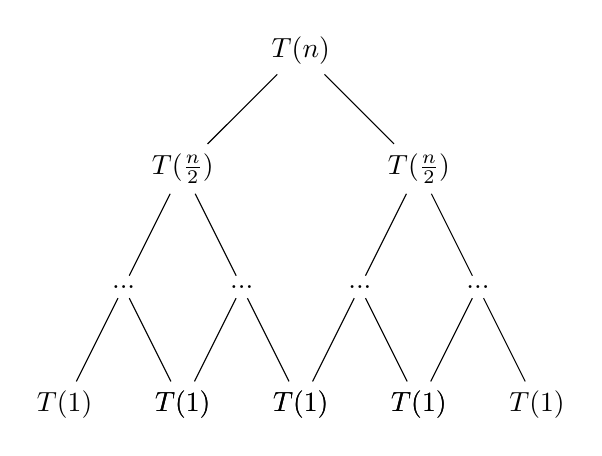
\begin{tikzpicture}[level distance=1.5cm,
  level 1/.style={sibling distance=3cm},
  level 2/.style={sibling distance=1.5cm}]
  \node {$T(n)$}
     child {node {$T(\frac{n}{2})$}
     child {node {$...$}   
     child {node {$T(1)$}}
     child {node {$T(1)$}}
    }
      child {node {$...$}
      child {node {$T(1)$}}
      child {node {$T(1)$}}}
    }
     child {node {$T(\frac{n}{2})$}
     child {node {$...$}
     child {node {$T(1)$}}
     child {node {$T(1)$}}}
     child {node {$...$}
     child {node {$T(1)$}}
     child {node {$T(1)$}}
     } 
     };
\end{tikzpicture} \\

\bigskip
\bigskip

This algorithm is essentially a modified version of merge sort. The array $A$ can be split up into individual columns, each of which is a leaf in the binary tree above. \\

The "merging" subroutine: To merge two length $n$ columns into a single sorted array, keep taking the largest element from either column until the merged array is complete (has length $2n$). This takes $\theta(n)$ time, because there are $n$ elements in each column. \\

At each layer of the tree, there are $\frac{m}{2^l}$ arrays to merge, where $l$ is the layer in the tree. However, the size of each array is $n \cdot 2^l$. So each layer will take the same amount of time to merge: $\theta(mn)$. \\

The height of the tree is $\log_2 m$, and each layer takes $\theta(mn)$ time, so the runtime will be $\theta(mn \cdot \log_2 m)$.



\end{problemparts}


\problem  % Problem 3

\begin{problemparts}
\problempart Part a % Problem 3a
\problempart Part b % Problem 3b
\problempart Part c % Problem 3c
\problempart Part d % Problem 3d
\end{problemparts}

\section*{Part B}

\problem
\begin{problemparts}
\problempart The following is an $O(n^2)$ algorithm that computes Bowser's final rank. Consider the pseudocode below:
\bigskip

losetimes =  \{ \}  \# this dictionary stores a key for each player, and a value for their losetime

\begin{tabbing}
for \= s in competitors: \\
	\> for \= f in competitors: \\
		\>\> min\_losetime = 1,000,000 \# initialized with a really high integer \\
		\>\> if \= s == f:\\
			\>\>\> continue\\
		\>\>else:\\
			\>\>\>if \=vel\_f $>$ vel\_s:\\
				\>\>\>\>time = calculate\_losetime(f, s)\\
				\>\>\>\>if \= time $<$ min\_losetime:\\
					\>\>\>\>\>min\_losetime = time\\
	\>losetimes[s] = min\_losetime\\
	\\
	\# increment bowser's rank every time a competitor is found with a longer finish time (meaning that they outlasted bowser)
	bowser\_rank = 1\\
	for\=time in losetimes.values():\\
		\>if \=time $>$ losetimes['bowser']:\\
			\>\>bowser\_rank += 1\\

\end{tabbing}



\problempart \emph{Submit your implementation on alg.csail.mit.edu}
\problempart \emph{Submit your implementation on alg.csail.mit.edu}
\problempart Part e % Problem 4e
\problempart \emph{Submit your implementation on alg.csail.mit.edu}
\end{problemparts}

\end{problems}

\end{document}

